\section{Opis struktury projektu}
\subsection{Architektura systemu}
System został zbudowany w oparciu o wzorzec MVC (Model-Widok-Kontroler):
\begin{itemize}
\item \textbf{Model}: Baza danych SQLite + klasy dziedziny (Produkt, Transakcja itp.)
\item \textbf{Widok}: Interfejs użytkownika zrealizowany w Swing
\item \textbf{Kontroler}: Logika biznesowa aplikacji
\end{itemize}

\subsection{Diagram klas}
\begin{figure}[H]
\centering
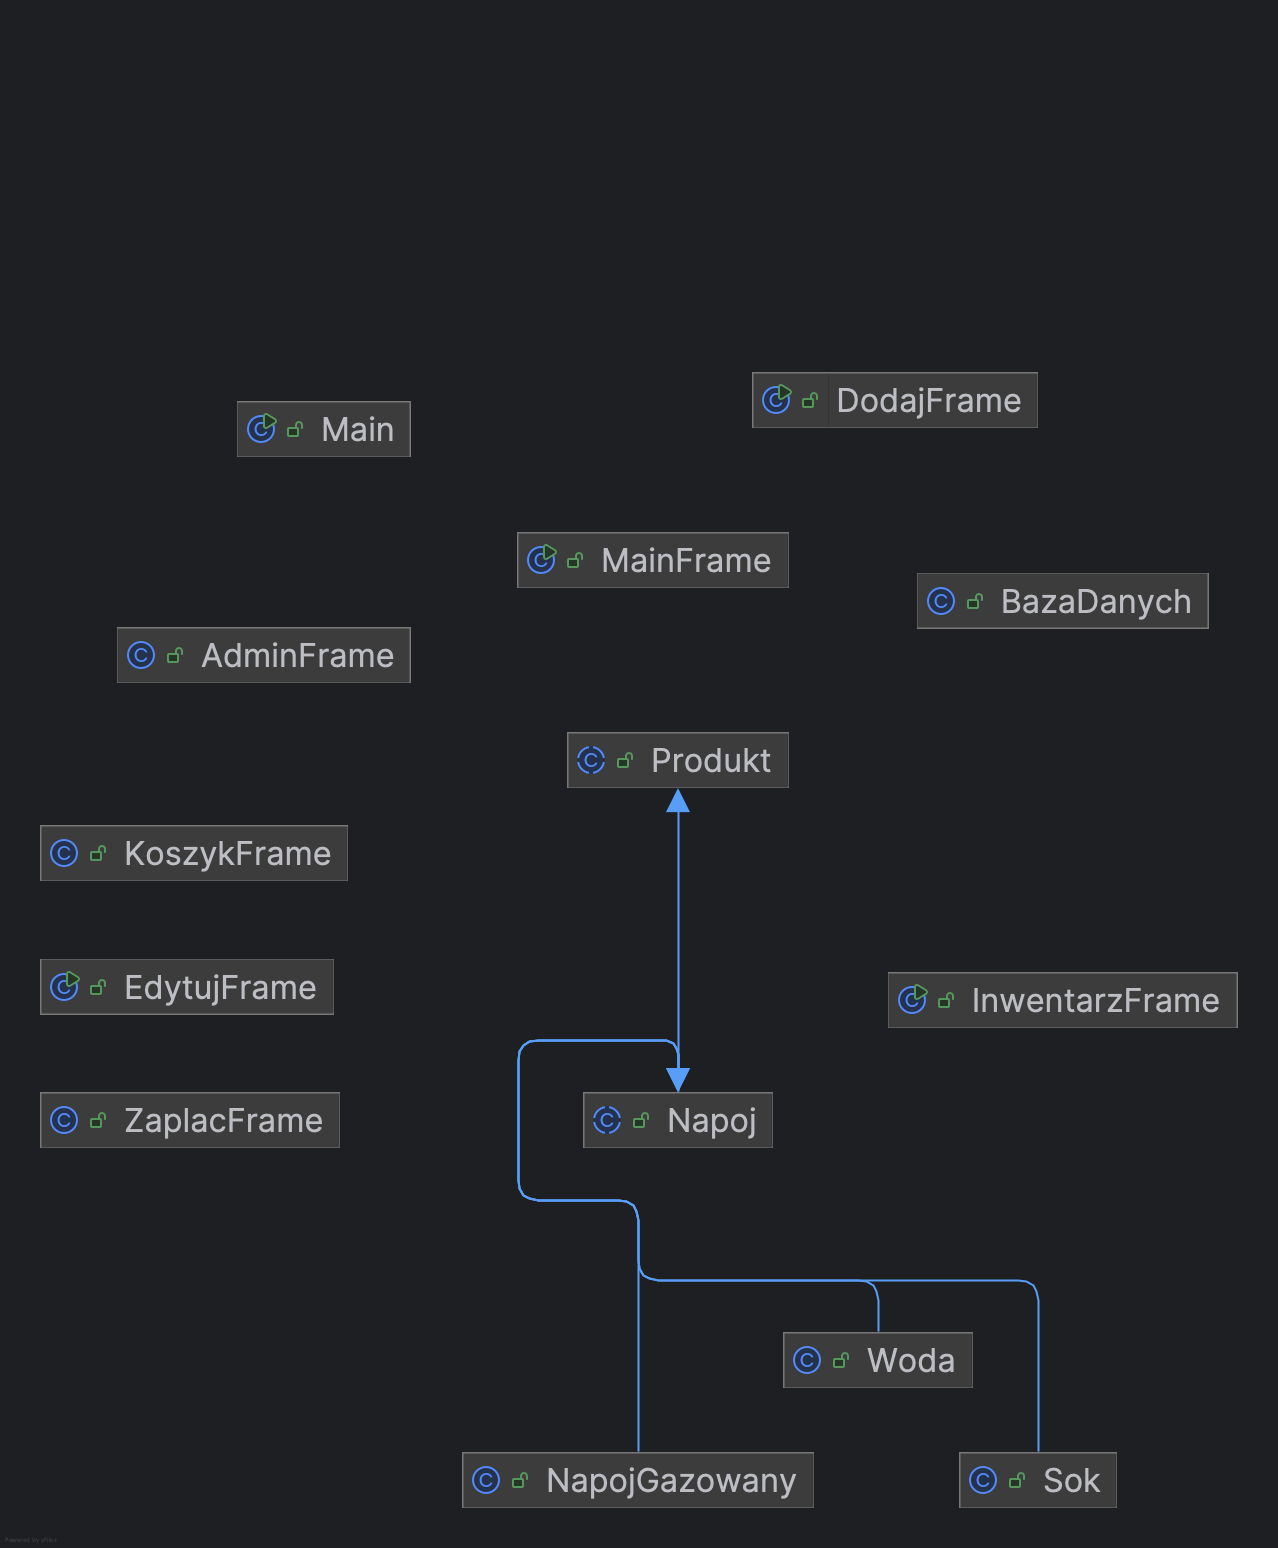
\includegraphics[width=0.9\textwidth]{figures/class_diagram.png}
\caption{Diagram głównych klas systemu}
\label{fig:class_diagram}
\end{figure}



Kluczowe klasy systemu:
\begin{itemize}
\item \textbf{MainFrame}: Główne okno aplikacji
\item \textbf{Produkt}: Klasa abstrakcyjna reprezentująca produkt
\item \textbf{Napoj}, \textbf{NapojGazowany}, \textbf{Woda}, \textbf{Sok}: Hierarchia klas produktów
\item \textbf{KoszykFrame}: Obsługa koszyka zakupowego
\item \textbf{ZaplacFrame}: Logika płatności
\item \textbf{BazaDanych}: Warstwa dostępu do danych
\end{itemize}


\subsection{Baza danych}
System wykorzystuje lekką bazę danych SQLite z następującymi tabelami:
\begin{itemize}
\item \textbf{produkty} (id, nazwa, cena, typ, ilość)
\item \textbf{detale\_napoje} (id\_produktu, pojemność\_ml)
\item \textbf{transakcje} (id, data, produkty, kwota, metoda\_płatności)
\end{itemize}

\begin{figure}[H]
\centering
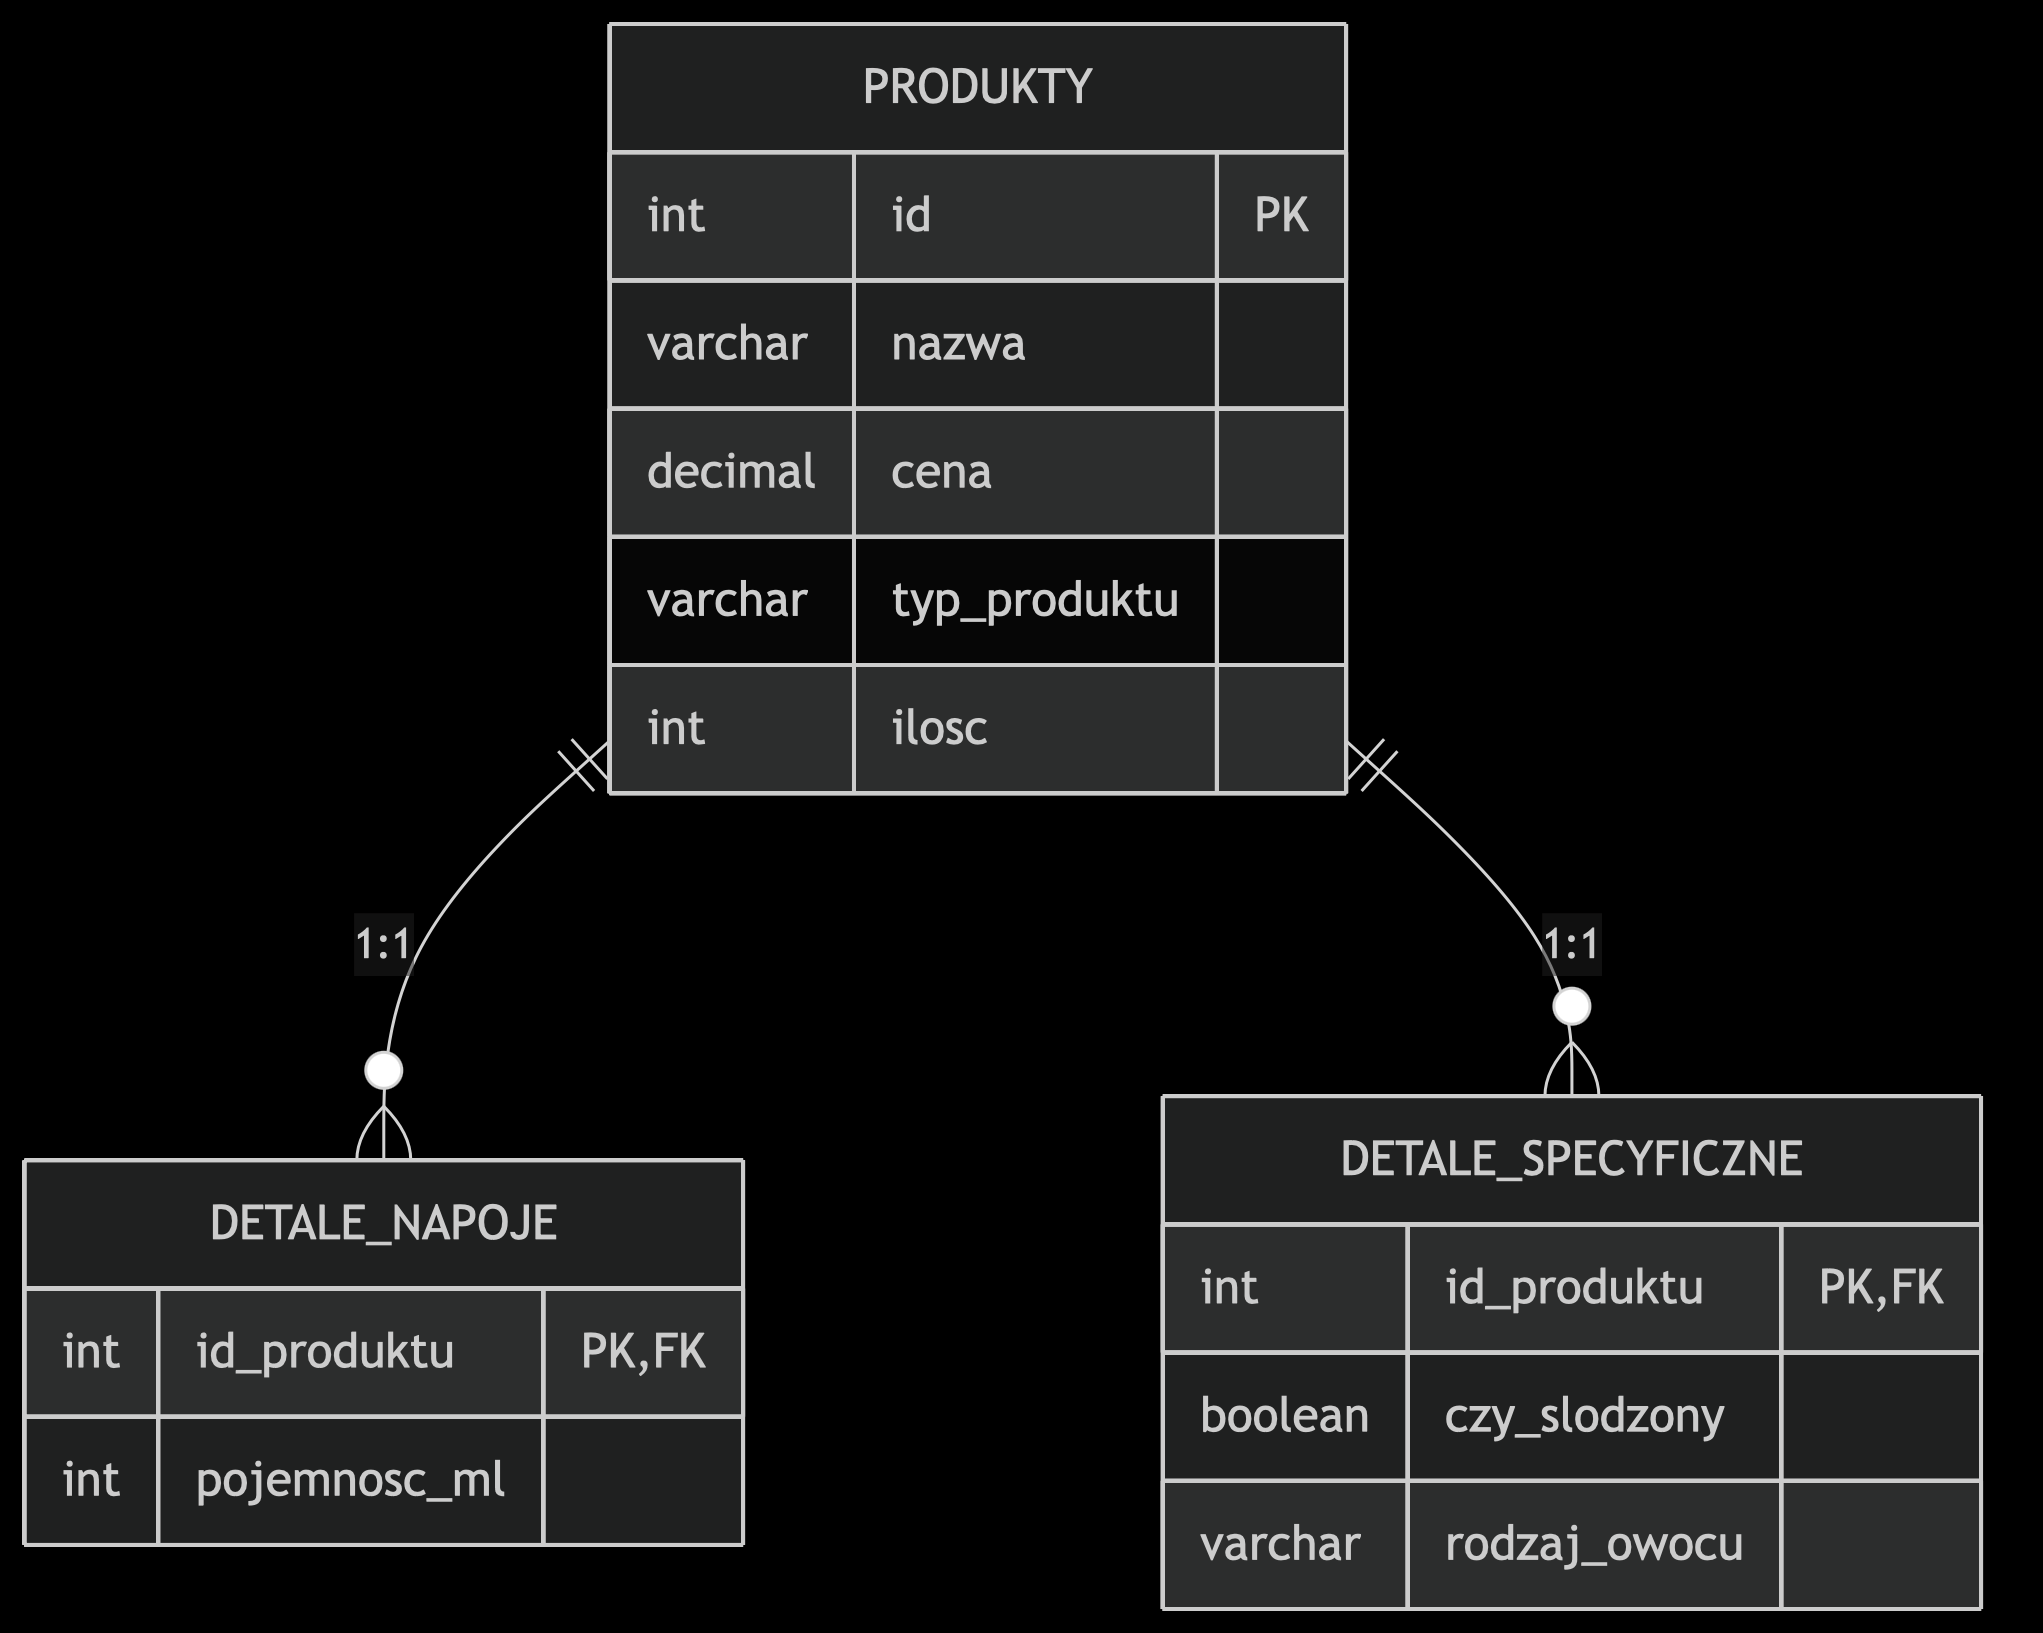
\includegraphics[width=0.8\textwidth]{figures/erd_diagram.png}
\caption{Diagram ERD bazy danych}
\label{fig:erd_diagram}
\end{figure}